% ---------------------------------------------------------------- 17
% [suite]
\begin{frame}{4.2 Comparer hors échantillon : l'idée du log-score prédictif}
\begin{columns}[t]
\begin{column}{0.50\textwidth}
\begin{kbox}[Principe]
Un modèle n'est pas jugé sur sa capacité à \emph{expliquer} les données
qu'il vient de voir (il peut toujours surenchérir en paramètres), mais sur sa
capacité à \textbf{prédire} une observation \emph{nouvelle}.
\[
\text{elpd} \;=\; \sum_{i=1}^{n} \log p(y_i \given y_{-i})
\]
« elpd » : \textit{expected log pointwise predictive density}, en nats.
Plus grand = mieux. $0$ = pas mieux qu'une prédiction au hasard calibrée.
\end{kbox}
\end{column}
\begin{column}{0.48\textwidth}
\begin{ebox}[Trois façons d'estimer l'elpd]
\begin{enumerate}
  \item \textbf{LOO-CV} : ajuster $n$ fois le modèle en retirant $y_i$,
        prédire $y_i$. Coût prohibitif, mais estimable par importance sampling.
  \item \textbf{DIC} : $\log p(y \given \bar\theta)$ pénalisé par le nombre
        effectif de paramètres $p_{DIC}$. Rapide, approximatif, suppose la
        normalité du posterior.
  \item \textbf{WAIC} : moyenne de $\log p(y_i \given \theta)$ sur le posterior,
        pénalisée par la variance de ces quantités. Aucune normalité requise.
\end{enumerate}
\end{ebox}
\end{column}
\end{columns}
\vspace{1mm}
\end{frame}

% [suite]
\begin{frame}{4.2 Comparer hors échantillon : l'idée du log-score prédictif (suite)}
\begin{tcolorbox}[colback=byCyan!8,colframe=byCyan,arc=2mm,width=.95\textwidth]
\small\centering
\textbf{Point clé} --- les trois critères estiment la \emph{même} espérance
(l'elpd) par trois biais et trois variances différents : ils peuvent
\textbf{désigner des vainqueurs différents}, surtout avec peu d'observations.
\end{tcolorbox}
\end{frame}

% ---------------------------------------------------------------- 18
\begin{frame}{DIC et WAIC : les formules, sans magie}
% [rogna]
\small
\begin{columns}[t]
\begin{column}{0.49\textwidth}
\begin{ebox}[DIC --- Deviance Information Criterion]
\[
p_{DIC} = 2\Big(\log p(y \given \bar\theta) - \E_{\post}\big[\log p(y \given \theta)\big]\Big)
\]
\[
DIC = -2\log p(y \given \bar\theta) + 2\,p_{DIC}
\]
$\bar\theta$ est la moyenne postérieure. $p_{DIC}$ mesure le \emph{coût}
du surajustement.
\end{ebox}
\begin{wbox}[Faiblesse du DIC]
Si le posterior est multimodal ou fortement asymétrique,
$\bar\theta$ n'est représentatif de rien : le DIC peut préférer le modèle
le plus flexible. Il suppose un posterior \textbf{approximativement gaussien}.
\end{wbox}
\end{column}
\begin{column}{0.49\textwidth}
\begin{ebox}[WAIC --- Widely Applicable IC]
\begin{align*}
\text{elpd}_{WAIC} = \sum_{i=1}^{n}\Big(&\log \E_{\post}[p(y_i \given \theta)]\\
&-\ \Var_{\post}[\log p(y_i \given \theta)]\Big)
\end{align*}
\[
WAIC = -2\,\text{elpd}_{WAIC}
\]
Le second terme est l'équivalent de $p_{DIC}$ : la \textbf{variance} des
log-vraisemblances point par point.
\end{ebox}
\begin{kbox}[Dans les deux cas]
Le critère est une \emph{deviance} : plus petit = mieux.
En pratique on ne calcule jamais WAIC à la main : \py{az.waic(idata)} après
\py{pm.compute\_log\_likelihood(idata)}.
\end{kbox}
\end{column}
\end{columns}
\end{frame}

% ---------------------------------------------------------------- 19
\begin{frame}{LOO-CV par PSIS : la référence, et ses avertissements}
% [rogna]
\small
\begin{columns}[t]
\begin{column}{0.51\textwidth}
\begin{kbox}[Estimation par importance sampling (PSIS)]
On ne réajuste \emph{pas} $n$ fois le modèle. On corrige les poids
postérieurs par le rapport de vraisemblance laissée de côté :
\[
\widehat{\text{elpd}}_{LOO} = \sum_{i=1}^{n}
\log\frac{\sum_{s} w_i^{s}\, p(y_i \given \theta^{s})}{\sum_{s} w_i^{s}},
\qquad w_i^{s} \propto \frac{1}{p(y_i \given \theta^{s})}
\]
Les queues de cette distribution de poids sont approchées par une loi de
Pareto généralisée.
\end{kbox}
\end{column}
\begin{column}{0.47\textwidth}
\begin{wbox}[L'avertissement qui compte : Pareto-$\hat k$]
Si $\hat k > 0{,}7$ pour une observation, son poids est instable et
l'elpd estimé n'est pas fiable.
\vspace{1mm}
\textbf{Résultat de notre exécution réelle} (8 équipes, 3 modèles, 500 tirages
par chaîne) :
\begin{itemize}
  \item M1 (regroupé) : $\hat k_{\max} = 0{,}540$ \ok
  \item M2 (indépendant) : $\hat k_{\max} = 0{,}889$ ; \textbf{6 observations
        sur 8} dépassent 0{,}67 \warn
  \item M3 (hiérarchique) : $\hat k_{\max} = 1{,}043$ ; \textbf{7 sur 8} \warn
\end{itemize}
ArviZ a émis les avertissements correspondants pendant l'exécution.
\end{wbox}
\end{column}
\end{columns}
\vspace{1mm}
\centering\small
Conséquence : avec $n = 8$ observations seulement, le classement par LOO reste
\textbf{fragile} ; c'est une raison de plus pour ne pas conclure sur un écart
inférieur à son erreur-type (slide 23).
\end{frame}

% ---------------------------------------------------------------- 20
% [rogna]
% [rogna]
% [rogna]
% [split]
\begin{frame}{WAIC, DIC, LOO sur trois modèles : la sortie de \py{az.compare}}
\begin{center}
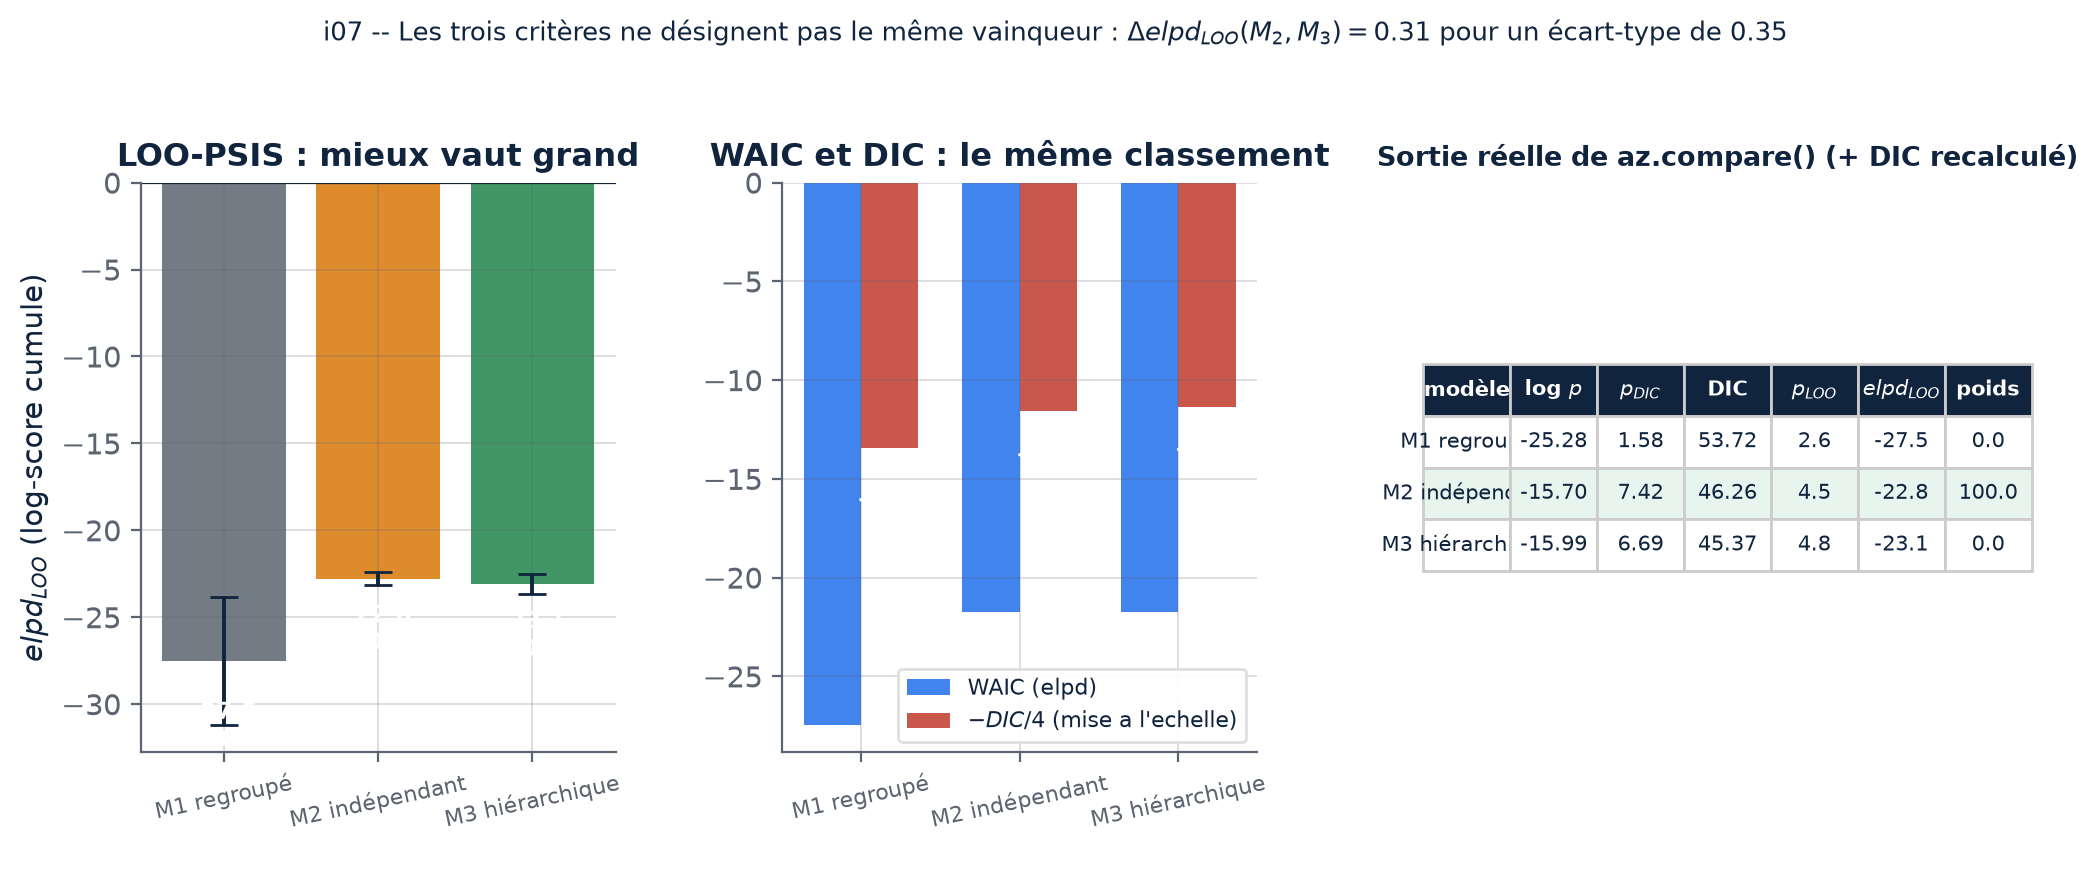
\includegraphics[width=.86\textwidth]{i07_waic_dic_loo.png}
\end{center}
\end{frame}

% [split]
\begin{frame}{WAIC, DIC, LOO sur trois modèles : la sortie de \py{az.compare}}

\vspace{-2mm}
\begin{columns}[t]
\begin{column}{0.52\textwidth}
\begin{ebox}[Données --- 8 équipes, $n_i$ entre 30 et 45 (lancé réellement)]
$y_i/n_i$ : $14/35$, $21/40$, $16/30$, $29/45$, $30/40$, $27/35$, $23/30$, $28/40$.
Trois modèles : M1 ($\theta$ commun), M2 ($\theta_i$ indépendants), M3 (hiérarchique :
$\theta_i \sim \mathrm{Beta}(\mu\kappa,(1{-}\mu)\kappa)$).
\end{ebox}
\end{column}
\begin{column}{0.46\textwidth}
\begin{solbox}[Ce que dit la sortie réelle]
\begin{itemize}
  \item \textbf{LOO} : M2 $-22{,}79$ (erreur-type $0{,}38$), M3 $-23{,}10$,
        M1 $-27{,}52$ ; poids $1{,}00$ / $0{,}00$ / $2{,}5\cdot10^{-16}$
  \item \textbf{WAIC} : M3 $-21{,}73$ (poids $0{,}608$), M2 $-21{,}73$
        (poids $0{,}392$), M1 $-27{,}48$
  \item \textbf{DIC} : M1 $53{,}72$, M2 $46{,}26$, M3 $45{,}37$
\end{itemize}
Les trois critères \textbf{ne désignent pas le même vainqueur}.
\end{solbox}
\end{column}
\end{columns}
\end{frame}

% ---------------------------------------------------------------- 21
\begin{frame}{L'elpd intra-échantillon triche : la correction est tout}
\begin{center}
\small
\begin{tabular}{@{}lrrrr@{}}
\toprule
Modèle & $p$ (params) & $\log p(y \given \bar\theta)$ \textit{in-sample} & $p_{eff}$ & $elpd_{LOO}$ \\
\midrule
M1 regroupé    & $1$ & $-25{,}28$ & $2{,}58$ & $-27{,}52$ \\
M2 indépendant & $8$ & $\mathbf{-15{,}70}$ \ok & $4{,}46$ & $\mathbf{-22{,}79}$ \\
M3 hiérarchique & $2 + 8$ & $-15{,}99$ & $4{,}85$ & $-23{,}10$ \\
\bottomrule
\end{tabular}
\end{center}
\vspace{1mm}
\begin{columns}[t]
\begin{column}{0.53\textwidth}
\begin{ebox}[Le renversement, chiffré]
En \emph{intra}-échantillon, M2 écrase M3 de $0{,}29$ nat et M1 de
$9{,}58$ nats. Après correction hors échantillon :
\[
\Delta(M_3, M_2) = 0{,}31 \quad (\text{dse} = 0{,}35),
\]
l'avance apparente de M2 a fondu de $9{,}58$ à $0{,}31$.
Et le nombre effectif de paramètres de M2 est $4{,}46$, pas $8$ : le
modèle indépendant est \emph{auto-régularisé} par son prior Beta$(1,1)$.
\end{ebox}
\end{column}
\begin{column}{0.45\textwidth}
\begin{kbox}[La règle de conduite]
\begin{itemize}
  \item Ne jamais classer des modèles sur $\log p(y \given \bar\theta)$ :
        cela récompense mécaniquement les paramètres en trop.
  \item Toujours regarder $p_{eff}$ : il n'est pas le nombre nominal de
        paramètres (M1 : $2{,}58$ pour $1$ paramètre, effet du prior ; M2 :
        $4{,}46$ pour $8$ paramètres, effet de la régularisation).
  \item Publier $elpd$, $p_{eff}$ et $\Delta \pm \text{dse}$.
\end{itemize}
\end{kbox}
\end{column}
\end{columns}
\end{frame}

% ---------------------------------------------------------------- 22
\begin{frame}{Trois critères en un tableau de décision}
\begin{center}
\footnotesize
\begin{tabular}{@{}p{2.3cm}p{2.9cm}p{3.0cm}p{3.4cm}@{}}
\toprule
& \textbf{DIC} & \textbf{WAIC} & \textbf{LOO-PSIS} \\
\midrule
Principe & deviance en $\bar\theta$ $+2p_{DIC}$ & log-score moyen $-$ pénalité de variance & log-score laissé-un-dehors par importance sampling \\[1mm]
Hypothèse & posterior gaussien & aucune & queues contrôlées \\[1mm]
Diagnostic & aucun & variance point par point & Pareto-$\hat k$ \\[1mm]
Coût & très faible & faible & modéré \\[1mm]
Nos 8 équipes & M3 ($45{,}37$) & M3 ($-21{,}73$) & M2 ($-22{,}79$) \\[1mm]
Verdict & utilitaire & bon compromis & \textbf{référence} \\
\bottomrule
\end{tabular}
\end{center}
\vspace{1mm}
\begin{kbox}[Comment choisir en pratique]
\textbf{LOO en premier} (avec ses diagnostics) ; \textbf{WAIC} pour un calcul
rapide et une confirmation ; \textbf{DIC} seulement pour comparer avec une
littérature ancienne ou pour de très grands modèles où LOO est impossible.
Si les trois divergent et que les écarts sont inférieurs à $2\,\text{dse}$ :
\textbf{ne pas trancher}, moyenner les prédictions.
\end{kbox}
\end{frame}

% ---------------------------------------------------------------- 23
% [rogna]
% [rogna]
% [rogna]
% [split]
\begin{frame}{Poids de modèles et moyennage prédictif}
\begin{center}
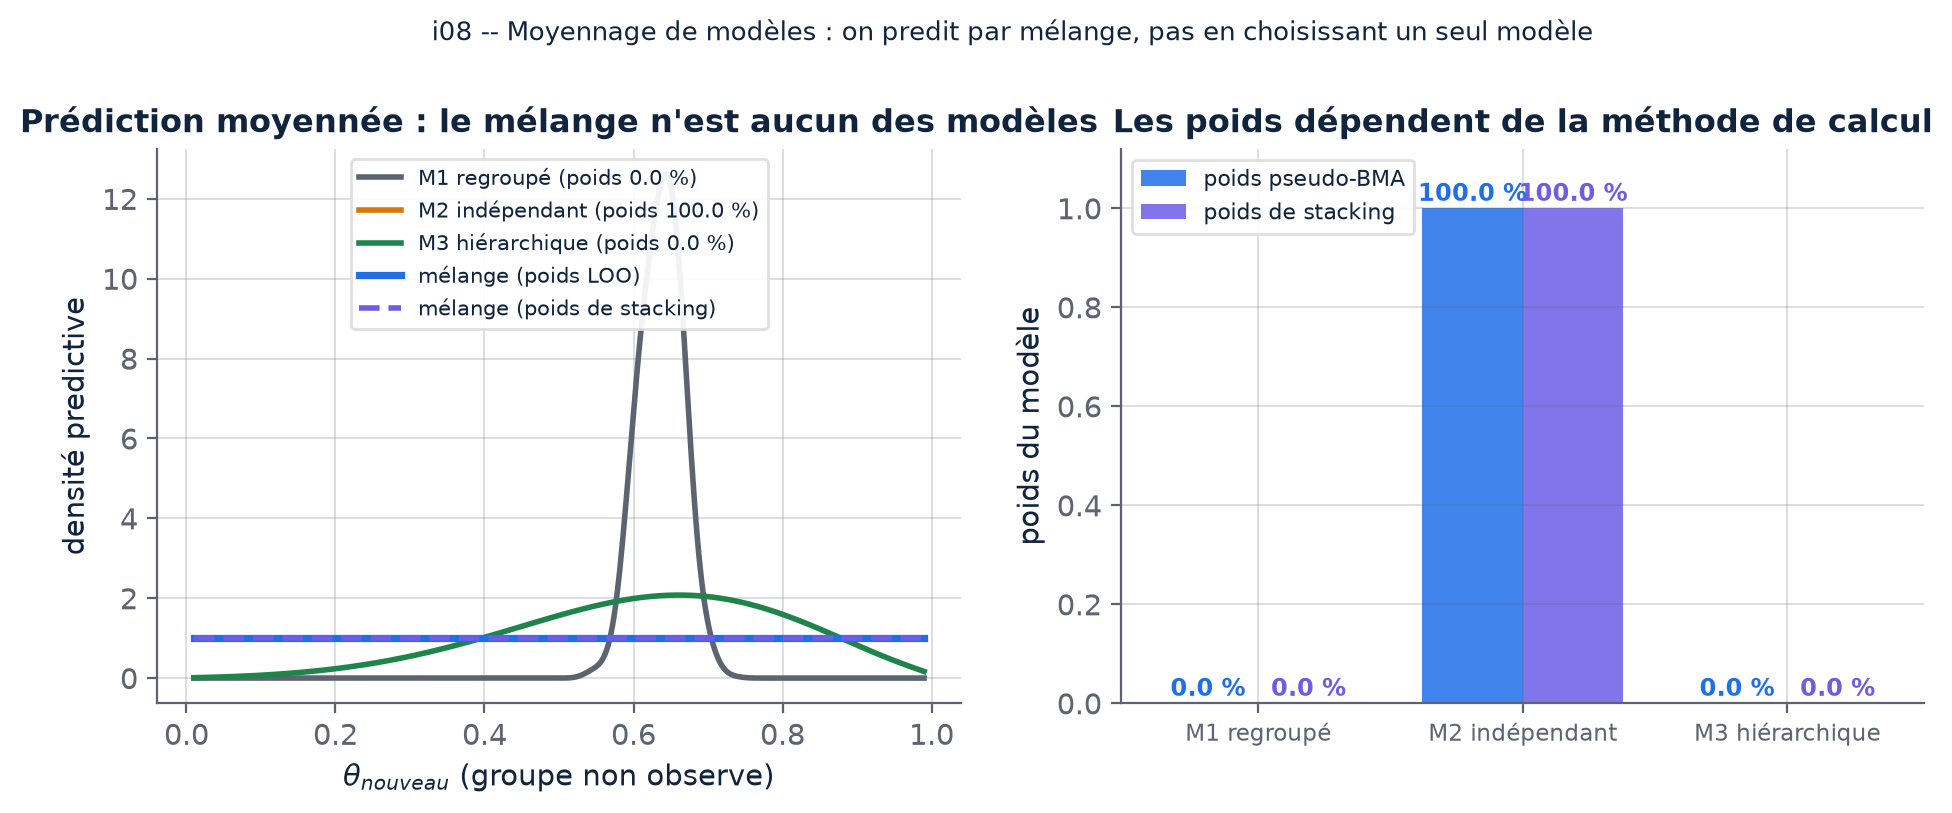
\includegraphics[width=.86\textwidth]{i08_model_averaging.png}
\end{center}
\end{frame}

% [split]
\begin{frame}{Poids de modèles et moyennage prédictif}

\vspace{-1mm}
\begin{columns}[t]
\begin{column}{0.52\textwidth}
\begin{kbox}[Le moyennage, pas le choix]
Pour prédire un nouveau groupe, on ne choisit pas un modèle : on \textbf{mélange}
les prédictives avec des poids issus des critères :
\[
p(\tilde y \given y) = \sum_{m} w_m\, p_m(\tilde y \given y)
\]
\end{kbox}
\begin{ebox}[Chiffres de l'exécution]
Poids LOO (pseudo-BMA) : M2 $=1{,}00$, M3 $=0{,}00$, M1 $=2{,}5\cdot10^{-16}$.
Poids de stacking : M2 $=1{,}00$.
Recouvrement entre la prédictive de M3 et le mélange : $0{,}674$.
\end{ebox}
\end{column}
\begin{column}{0.46\textwidth}
\begin{wbox}[Le piège des poids dégénérés]
Quand deux modèles sont \textbf{indiscernables} ($\Delta = 0{,}31$ pour
$\text{dse} = 0{,}35$), la formule des poids pseudo-BMA attribue
$1{,}00$ et $0{,}00$ : c'est un artefact, pas une information.
\vspace{1mm}
\footnotesize Remèdes : moyennage par \emph{stacking} (plus stable),
prédiction conjointe de plusieurs modèles, ou modèle hiérarchique
englobant les deux (le plus honnête quand c'est possible).
\end{wbox}
\end{column}
\end{columns}
\end{frame}

% ---------------------------------------------------------------- 22
\begin{frame}[fragile]{Le code réel de la comparaison (PyMC + ArviZ)}
\begin{columns}[t]
\begin{column}{0.56\textwidth}
\begin{codebox}[compare\_models.py --- extrait exécuté en TP]
\begin{lstlisting}[style=py]
import pymc as pm, arviz as az

with pm.Model() as m3:                # modele hierarchique
    mu    = pm.Beta("mu", 2, 2)
    kappa = pm.HalfNormal("kappa", 5)
    theta = pm.Beta("theta", mu*kappa, (1-mu)*kappa,
                    shape=8)
    pm.Binomial("y", n=n_obs, p=theta, observed=y_obs)
    idata3 = pm.sample(draws=500, tune=500,
                       chains=2, cores=1)
    pm.compute_log_likelihood(idata3)   # OBLIGATOIRE

cmp = az.compare({"M1": idata1, "M2": idata2, "M3": idata3},
                 ic="loo", method="stacking")
print(cmp[["rank","elpd_loo","p_loo",
           "elpd_diff","dse","weight"]])
\end{lstlisting}
\end{codebox}
\end{column}
\begin{column}{0.42\textwidth}
\begin{solbox}[Sortie réelle (tronquée)]
\footnotesize
\begin{tabular}{@{}lrrr@{}}
\toprule
modèle & $elpd_{LOO}$ & $p_{LOO}$ & poids \\
\midrule
M2 & $-22{,}79$ & $4{,}46$ & $1{,}00$ \\
M3 & $-23{,}10$ & $4{,}85$ & $0{,}00$ \\
M1 & $-27{,}52$ & $2{,}58$ & $0{,}00$ \\
\bottomrule
\end{tabular}
\vspace{1.5mm}
$\Delta(M_3,M_2) = 0{,}31$, $\text{dse} = 0{,}35$ : \textbf{indécelable}.
\end{solbox}
\begin{kbox}[Deux réflexes de code]
\begin{itemize}
  \item \py{pm.compute\_log\_likelihood} \textbf{avant} tout \py{az.compare},
        sinon ArviZ ne peut rien calculer.
  \item Toujours afficher \py{dse} (erreur-type de la différence) :
        un $\Delta$ seul ne veut rien dire.
\end{itemize}
\end{kbox}
\end{column}
\end{columns}
\end{frame}

% ---------------------------------------------------------------- 23
\begin{frame}{Avertissements : ce qu'un critère ne dit pas}
% [rogna]
\small
\begin{columns}[t]
\begin{column}{0.49\textwidth}
\begin{wbox}[Cinq pièges de la comparaison de modèles]
\begin{itemize}
  \item \textbf{Modèles emboîtés} : comparer $M_1 \subset M_3$ par un critère
        hors échantillon n'est pas un test de $H_0$ ; l'écart est
        \emph{biaisé} en faveur du plus grand modèle.
  \item \textbf{Écart non significatif} : $\Delta = 0{,}31$ pour
        $\text{dse} = 0{,}35$ : aucune conclusion. Il faut
        $|\Delta| > 2\,\text{dse}$ pour parler de différence.
  \item \textbf{Poids de modèles} : ils ne sont pas des probabilités
        postérieures de modèle (pas de prior sur les modèles) : ne dites pas
        « M2 a 100\,\% de chance d'être le vrai modèle ».
  \item \textbf{Pareto-$\hat k$} : $\hat k_{\max} = 1{,}043$ pour M3 :
        l'elpd de M3 est une estimation instable.
  \item \textbf{$n$ petit} : le classement est instable ; refaites-le
        avec un autre découpage ou un autre seed.
\end{itemize}
\end{wbox}
\end{column}
\begin{column}{0.49\textwidth}
\begin{kbox}[Bonnes pratiques 2026]
\begin{enumerate}
  \item Calculer \textbf{toujours} \py{az.loo} \emph{et} \py{az.waic} :
        s'ils divergent, le doute est légitime.
  \item Publier le tableau complet (elpd, $p_{eff}$, $\Delta$, dse, poids).
  \item Vérifier les diagnostics d'échantillonnage ($\hat R$, ESS,
        divergences) \emph{avant} de comparer : un modèle mal échantillonné
        a un mauvais elpd pour de mauvaises raisons.
  \item Rapporter la sensibilité aux priors des modèles concurrents.
  \item Ne pas transformer un critère en décision : passer à la section 4.3.
\end{enumerate}
\end{kbox}
\end{column}
\end{columns}
\end{frame}

% ---------------------------------------------------------------- 24
% [suite]
\begin{frame}{4.3 Décision bayésienne : perte, action, risque}
\begin{kbox}[Le vocabulaire, fixé une fois pour toutes]
\begin{itemize}
  \item \textbf{Action} $a \in \mathcal{A}$ : ce qu'on décide de faire (traiter,
        déployer B, publier, rétrograder un modèle\dots).
  \item \textbf{Perte} $L(\theta, a)$ : le coût encouru si la vérité est
        $\theta$ et qu'on agit selon $a$. On l'écrit en euros, en vies,
        en heures perdues --- jamais en probabilité.
  \item \textbf{Risque a posteriori} : la perte moyenne sous le posterior,
        \[
        \rho(a) = \E_{\theta \given y}\big[L(\theta,a)\big]
        = \int L(\theta,a)\,\pi(\theta \given y)\,\mathrm{d}\theta .
        \]
  \item \textbf{Décision bayésienne} : $a^\star = \argmin_{a} \rho(a)$.
\end{itemize}
\end{kbox}
\vspace{1mm}
\end{frame}

% [suite]
\begin{frame}{4.3 Décision bayésienne : perte, action, risque (suite)}
\begin{columns}[t]
\begin{column}{0.49\textwidth}
\begin{ebox}[Pourquoi c'est la bonne façon de poser le problème]
Le posterior contient \emph{tout} ce qu'on sait ; la perte contient tout
ce qui compte. Séparer les deux évite les débats stériles : le statisticien
fournit $\pi(\theta \given y)$, le décideur fournit $L$.
\end{ebox}
\end{column}
\begin{column}{0.49\textwidth}
\begin{wbox}[Le piège du « seuil à 0,95 »]
Exiger $P(\theta > 0) > 0{,}95$ pour agir \emph{est} une règle de décision,
mais avec une perte implicite $0$--$1$ et un seuil jamais discuté.
Combien coûte une erreur dans chaque sens ? Si la réponse est « pas pareil »,
le seuil 0,95 est faux.
\end{wbox}
\end{column}
\end{columns}
\end{frame}

% ---------------------------------------------------------------- 25
\begin{frame}{Trois pertes, trois estimateurs, trois décisions}
\begin{center}
\small
\begin{tabular}{@{}p{3.4cm}p{4.2cm}rr@{}}
\toprule
\textbf{Perte} $L(\theta,a)$ & \textbf{Décision optimale} & \textbf{Valeur sur Beta}(3,7) & \textbf{Type} \\
\midrule
$(\theta - a)^2$ (quadratique) & la \textbf{moyenne} postérieure & $0{,}3001$ & estimation \\
$|\theta - a|$ (absolue) & la \textbf{médiane} postérieure & $0{,}2858$ & estimation \\
0--1 symétrique & la \textbf{région de masse dominante} & seuil $0{,}5000$ & décision \\
asymétrique $c_{fn}/c_{fp} = 19$ & le seuil $q = \frac{c_{fp}}{c_{fp}+c_{fn}}$ & $q = 0{,}0500$ & décision \\
\bottomrule
\end{tabular}
\end{center}
\vspace{1mm}
\begin{columns}[t]
\begin{column}{0.49\textwidth}
\begin{ebox}[Vérifié : analytique contre numérique]
Sur le posterior $\mathrm{Beta}(3,7)$ et une grille fine, on cherche par
minimisation numérique le seuil optimal :
\[
\text{argmin} = 0{,}5006 \; / \; 0{,}1999 \; / \; 0{,}0997 \; / \; 0{,}0502
\]
pour $c_{fn}/c_{fp} = 1 / 4 / 9 / 19$, à comparer aux valeurs analytiques
$0{,}50$, $0{,}20$, $0{,}10$, $0{,}05$. \ok
\end{ebox}
\end{column}
\begin{column}{0.49\textwidth}
\begin{kbox}[Ce qu'il faut retenir]
\begin{itemize}
  \item La moyenne minimise le risque quadratique, la médiane le risque absolu.
  \item Pour une \emph{décision} binaire, le seuil sur $\theta$ est
        $\frac{\text{coût d'un faux positif}}{\text{somme des deux coûts}}$ :
        \textbf{indépendant du posterior}.
  \item Le posterior ne change donc pas le \emph{seuil} d'une décision binaire :
        il détermine de quel côté du seuil on tombe.
\end{itemize}
\end{kbox}
\end{column}
\end{columns}
\end{frame}

% ---------------------------------------------------------------- 26
% [rogna]
% [rogna]
% [rogna]
% [split]
\begin{frame}{Risque a posteriori et seuil optimal selon le rapport de coûts}
\begin{center}
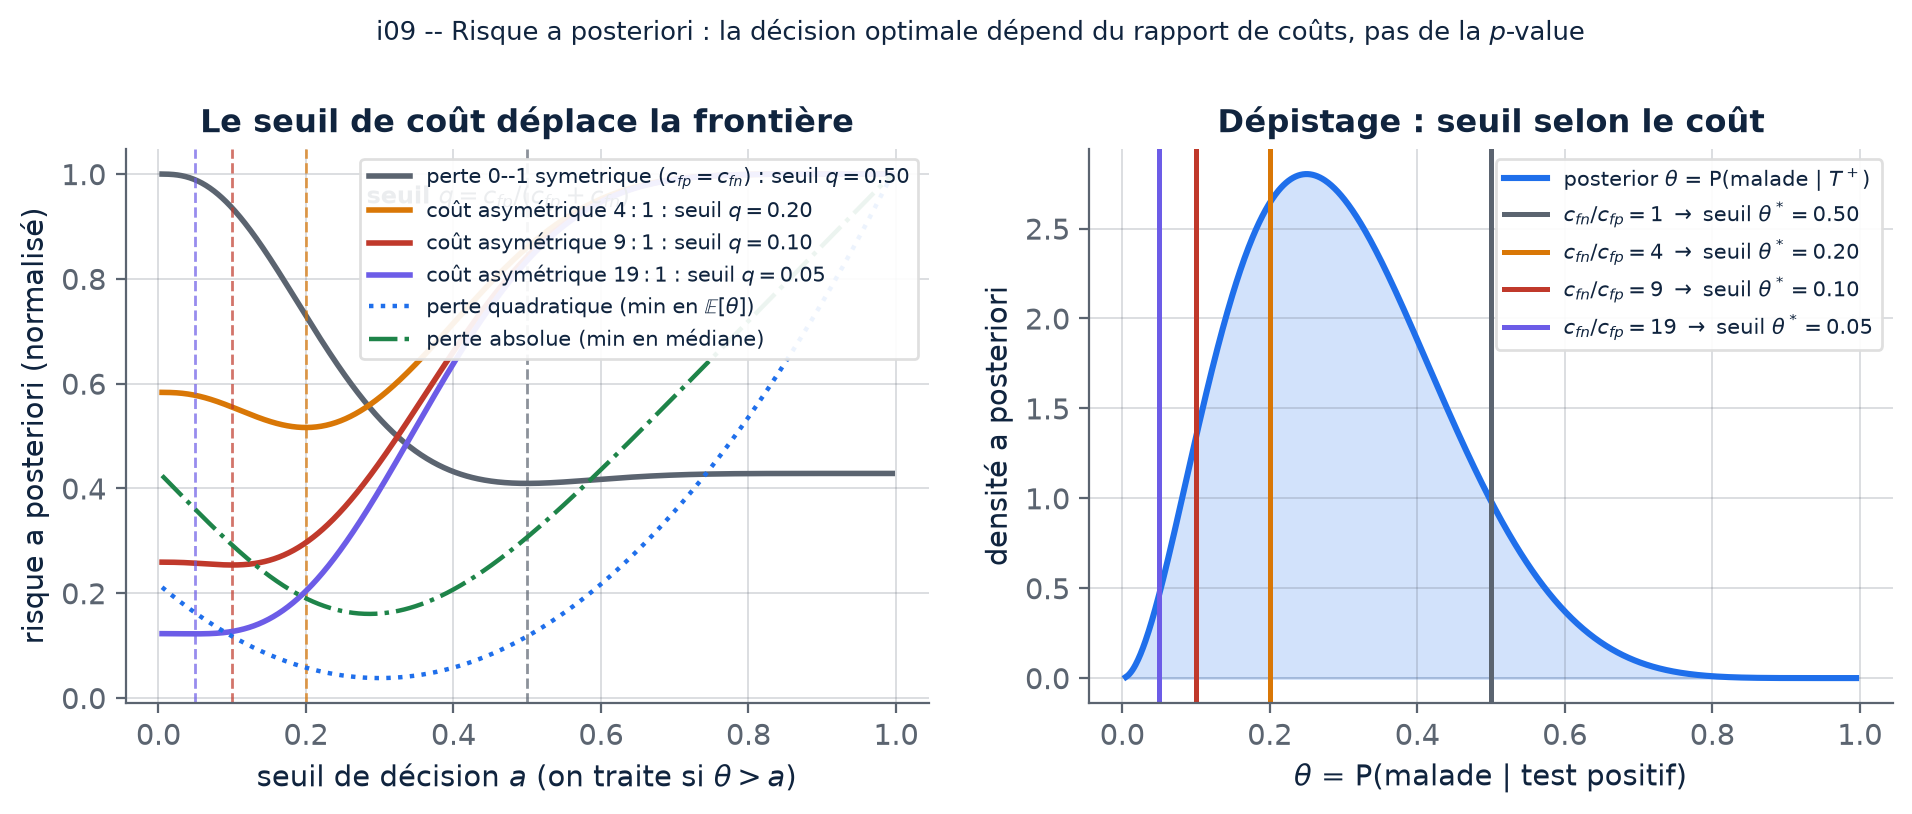
\includegraphics[width=.86\textwidth]{i09_risk_threshold.png}
\end{center}
\end{frame}

% [split]
\begin{frame}{Risque a posteriori et seuil optimal selon le rapport de coûts}

\vspace{-1mm}
\begin{columns}[t]
\begin{column}{0.53\textwidth}
\begin{ebox}[Dépistage, exécuté sur un posterior $\mathrm{Beta}(3,7)$]
$\theta = P(\text{malade} \given T^+)$, moyenne $0{,}300$.
\begin{itemize}
  \item $c_{fn}/c_{fp} = 1$ : seuil $0{,}50$, risque minimal $0{,}287$
        ($P(\theta>0{,}5) = 0{,}090$)
  \item $c_{fn}/c_{fp} = 4$ : seuil $0{,}20$, risque $0{,}620$
        ($P(\theta>0{,}2) = 0{,}738$)
  \item $c_{fn}/c_{fp} = 9$ et $19$ : seuils $0{,}10$ et $0{,}05$,
        risques $0{,}685$ et $0{,}698$
\end{itemize}
\end{ebox}
\end{column}
\begin{column}{0.45\textwidth}
\begin{wbox}[Un seul nombre ne suffit pas]
$P(\text{malade} \given T^+) = 0{,}09$ ne dit pas s'il faut traiter.
Avec un coût de maladie grave $19\times$ supérieur au coût du traitement
inutile, \textbf{on traite} : le seuil tombe à $0{,}05$ et la probabilité
postérieure le dépasse.
\vspace{1mm}
\footnotesize En fréquentiste, la conclusion serait la même « p-value » dans
les quatre cas : seul le calculateur de coûts change la réponse.
\end{wbox}
\end{column}
\end{columns}
\end{frame}

% ---------------------------------------------------------------- 27
\begin{frame}{Le seuil optimal se dérive analytiquement}
\begin{columns}[t]
\begin{column}{0.52\textwidth}
\begin{solbox}[Dérivation complète (3 lignes)]
Décision : agir ($\theta > a$) ou s'abstenir.
\[
\rho(a) = c_{fn}\,\E[\theta\,\mathbf{1}_{\theta \le a}]
        + c_{fp}\,\E[(1-\theta)\,\mathbf{1}_{\theta > a}]
\]
\[
\frac{\partial \rho}{\partial a}
= f(a)\Big[c_{fn}\,a - c_{fp}(1-a)\Big] = 0
\]
\[
\boxed{\;a^\star = \frac{c_{fp}}{c_{fp}+c_{fn}}\;}
\]
Le seuil ne dépend \textbf{ni} du posterior \textbf{ni} de $n$ : seulement
du rapport des coûts.
\end{solbox}
\end{column}
\begin{column}{0.46\textwidth}
\begin{qbox}[Question éclair (2 min)]
Un test coûte 30~€ et un cancer manqué coûte 30\,000~€ en espérance.
Quel doit être le seuil de probabilité postérieure pour agir ?
\vspace{2mm}
\begin{enumerate}
  \item[(A)] $0{,}95$ \quad (la tradition)
  \item[(B)] $0{,}001$ \quad \checkmark
  \item[(C)] $0{,}50$
  \item[(D)] cela dépend du posterior
\end{enumerate}
\vspace{2mm}
\textcolor{byBlue}{\textbf{Solution.}} $a^\star = 30/(30+30\,000) = 0{,}000999$ :
on agit dès que la probabilité dépasse \textbf{0,1\,\%}.
C'est parce que le coût de l'abstention est $1\,000$ fois plus grand que
celui de l'action inutile.
\end{qbox}
\end{column}
\end{columns}
\end{frame}

% ---------------------------------------------------------------- 28
\begin{frame}{ROPE : décider à trois issues}
\begin{columns}[t]
\begin{column}{0.52\textwidth}
\begin{kbox}[Region of Practical Equivalence]
La ROPE est l'intervalle $[-\delta,\delta]$ des effets \textbf{sans intérêt
pratique}. On calcule trois probabilités postérieures :
\[
P(\Delta < -\delta),\quad P(\Delta \in \mathrm{ROPE}),\quad P(\Delta > \delta)
\]
Règle usuelle (Kruschke) : si $P(\Delta \in \mathrm{ROPE}) > 0{,}95$
$\Rightarrow$ équivalence pratique ; si $P(\Delta > \delta) > 0{,}95$
$\Rightarrow$ supériorité ; \textbf{sinon} : indécis, continuer la collecte.
\end{kbox}
\begin{ebox}[Exemple exécuté, ROPE $= \pm 0{,}005$]
$n = 5\,000$ par bras, 500 contre 502 conversions
($\Delta$ observé $= +0{,}04$ point) :
\[
P(\Delta < -0{,}005) = 0{,}185,\quad
P(\Delta \in \mathrm{ROPE}) = 0{,}594,\quad
P(\Delta > 0{,}005) = 0{,}222
\]
\end{ebox}
\end{column}
\begin{column}{0.46\textwidth}
\begin{center}
\begin{figbox}
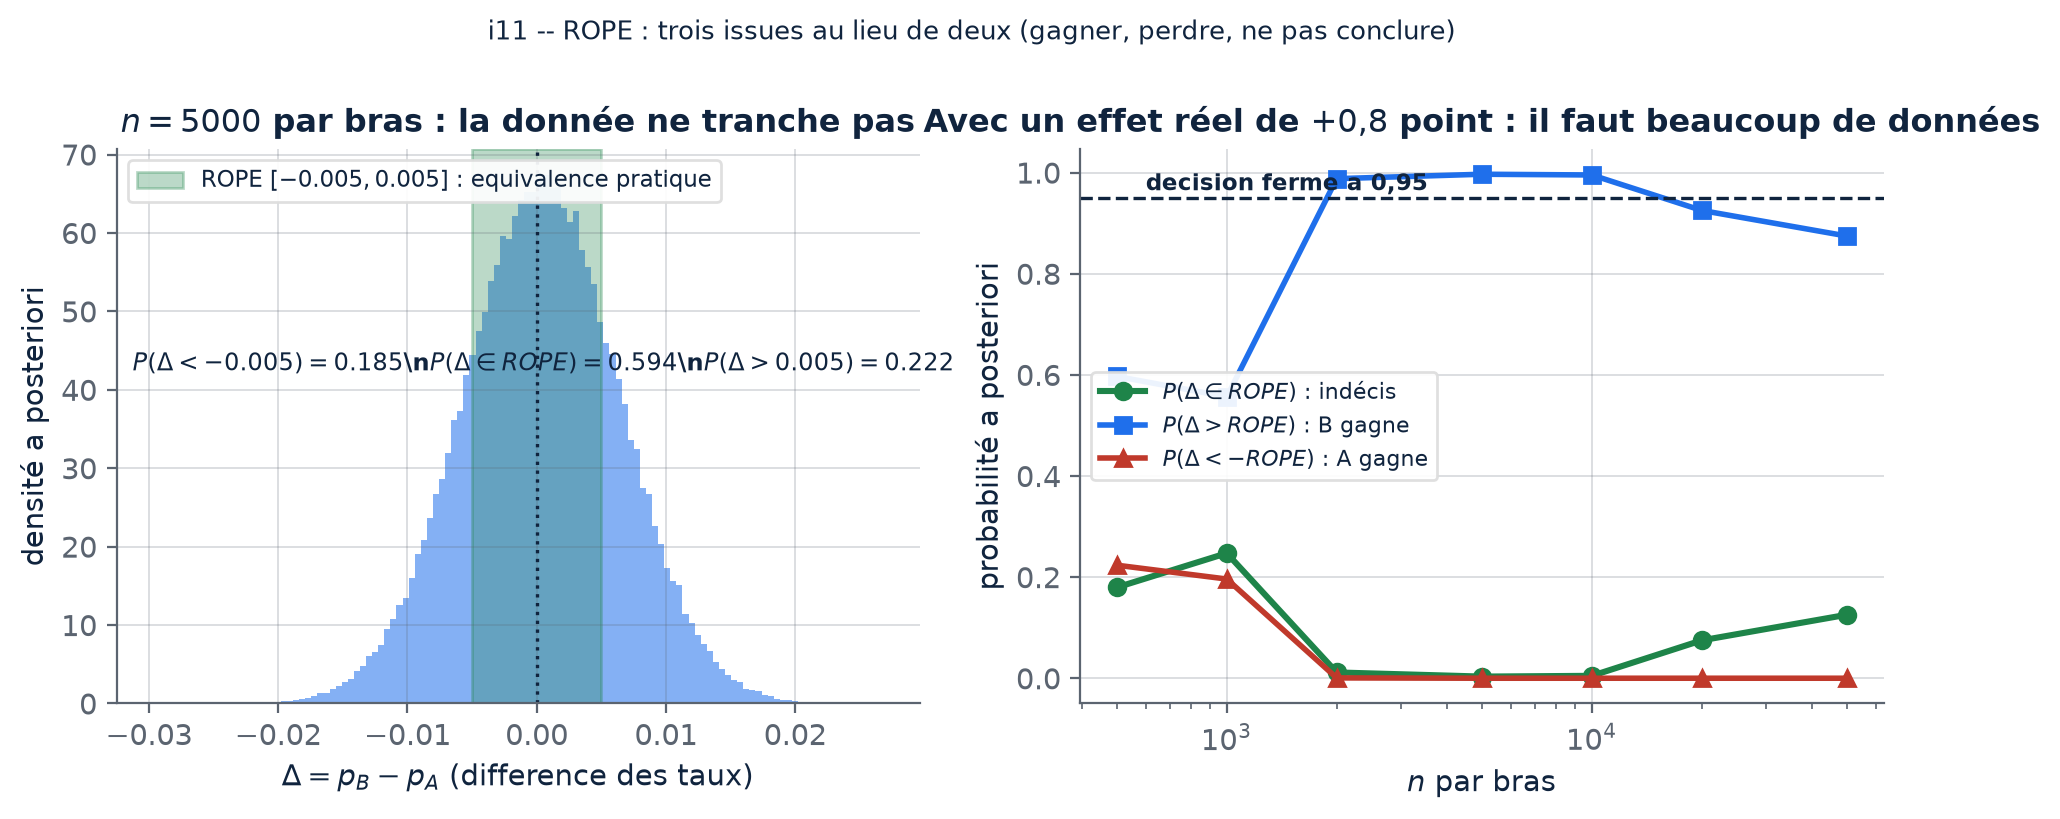
\includegraphics[width=\textwidth]{i11_rope.png}
\end{figbox}
\end{center}
\begin{wbox}[Effet réel minuscule : patience]
Avec un effet vrai de $+0{,}8$ point et une ROPE de $\pm0{,}5$ point,
50\,000 visiteurs par bras donnent encore
$P(\Delta > \mathrm{ROPE}) = 0{,}874$ : \textbf{faux espoir} de conclure vite.
\end{wbox}
\end{column}
\end{columns}
\end{frame}

% ---------------------------------------------------------------- 29
\begin{frame}{Choisir $\delta$ : le seul paramètre vraiment subjectif}
% [rogna]
\small
\begin{columns}[t]
\begin{column}{0.49\textwidth}
\begin{kbox}[Trois façons de fixer $\delta$]
\begin{itemize}
  \item \textbf{Métier} : « un gain de conversion inférieur à 0,5 point ne
        rembourse pas la complexité technique » $\Rightarrow \delta = 0{,}005$.
  \item \textbf{Résolution de l'instrument} : $\delta = $ la plus petite
        différence que la mesure sait distinguer.
  \item \textbf{Référence à un effet connu} : $\delta = 0{,}1 \times$ l'effet
        des actions passées.
\end{itemize}
\end{kbox}
\vspace{1mm}
\begin{ebox}[La ROPE change le \emph{sens} de la décision]
Sans ROPE, « ne pas rejeter » se confond avec « pas d'effet ».
Avec ROPE, on distingue :
\textbf{(1)} équivalence pratique démontrée, \textbf{(2)} différence
démontrée, \textbf{(3)} données insuffisantes pour trancher.
\end{ebox}
\end{column}
\begin{column}{0.49\textwidth}
\begin{wbox}[ROPE $\ne$ IC à 95\,\%]
\begin{itemize}
  \item L'IC à 95\,\% décrit \emph{où est} $\Delta$.
  \item La ROPE décrit \emph{ce qui compte}.
  \item Un IC qui chevauche la ROPE $\ne$ une équivalence : il faut la
        \emph{probabilité de masse} dans la ROPE, pas un recouvrement
        d'intervalles (même piège qu'au slide 5 avec le $BF$).
\end{itemize}
\end{wbox}
\begin{kbox}[Toujours annoncer $\delta$]
Écrivez $\delta$ dans le protocole \emph{avant} de voir les données :
c'est la version moderne de la préinscription.
\end{kbox}
\end{column}
\end{columns}
\end{frame}

% ---------------------------------------------------------------- 30
\begin{frame}{Quiz 2 --- perte, risque et décision}
\begin{qbox}[Question 1 --- depistage (5 min)]
Un test revient positif. Le posterior donne $P(\text{malade} \given T^+) = 0{,}09$.
Le traitement coûte l'équivalent de 1 unité ; rater la maladie coûte 9 unités.
Que fait-on ?
\vspace{2mm}
\begin{enumerate}
  \item[(A)] On ne traite pas : 9\,\% c'est trop faible
  \item[(B)] On traite : le seuil est $1/(1+9) = 0{,}10$ \dots\ on hésite \checkmark
  \item[(C)] On traite : le seuil est 0,95
  \item[(D)] On demande une $p$-value
\end{enumerate}
\vspace{2mm}
\textcolor{byBlue}{\textbf{Solution.}} Le seuil est $q = c_{fp}/(c_{fp}+c_{fn}) = 1/10 = 0{,}10$,
et $P(\text{malade} \given T^+) = 0{,}0898 < 0{,}10$ : de justesse, on
\emph{ne traite pas} --- mais la décision basculerait avec un coût de 9,5 unités.
Voilà pourquoi la discussion du coût est un acte statistique.
\end{qbox}
\vspace{1mm}
\begin{kbox}[Question 2 --- moyenne ou médiane ?]
« Le coût de l'erreur est proportionnel au carré de l'écart »
$\Rightarrow$ rapportez la \textbf{moyenne}\\
« Le coût est proportionnel à l'écart absolu » $\Rightarrow$ rapportez la
\textbf{médiane}\\
« Rien à cirer de 2\,\% d'écart, mais 20\,\% c'est grave » $\Rightarrow$ la
ROPE et une \textbf{décision à trois issues}.
\end{kbox}
\end{frame}

% ---------------------------------------------------------------- 31
\begin{frame}{Activité --- du posterior à la décision (TD, 20 min)}
% [rogna]
\small
\begin{abox}[Énoncé]
Une usine mesure la résistance moyenne d'un lot de câbles,
$\theta \sim \mathcal{N}(m, s^2)$ après les mesures. Deux actions :
livrer le lot ($a_0$) ou le recycler ($a_1$).
\begin{itemize}
  \item Recycler un lot conforme coûte $c_{fp} = 4\,000$~€.
  \item Livrer un lot non conforme coûte $c_{fn} = 60\,000$~€.
  \item On suppose le posterior de la proportion de conformité $\theta$
        disponible sous forme d'échantillon (\py{idata}).
\end{itemize}
\vspace{1mm}
\begin{enumerate}
  \item Quelle est la perte à utiliser ? Quelle est la décision optimale en
        fonction de $P(\theta > \text{seuil} \given y)$ ?
  \item Calculer le seuil analytique et l'écrire comme une fonction des coûts.
  \item Avec un échantillon postérieur simulé, estimer le risque des deux
        actions et vérifier $\argmin$.
\end{enumerate}
\end{abox}
\vspace{1mm}
\begin{solbox}[Solution attendue]
$a^\star = 4\,000/(4\,000+60\,000) = 0{,}0625$ : on \textbf{recycle} dès que la
probabilité de non-conformité dépasse $6{,}25\,\%$. Le risque estimé
numériquement sur 20\,000 tirages postérieurs doit donner le même argmin,
aux erreurs de Monte-Carlo près (à vérifier en séance).
\end{solbox}
\end{frame}
